\documentclass[landscape,border={0cm 0cm 0.5cm 1cm}]{standalone}

\usepackage{amssymb}
\usepackage{amsmath}
\usepackage{tikz}
\usetikzlibrary{calc}					%for centerarc
\usetikzlibrary{shadings}				%for diagonal shading (solid bullet)
\usetikzlibrary{arrows, arrows.meta}	%for white arrow
\usetikzlibrary{shapes.geometric}		%for hexagons
\usetikzlibrary{shapes.symbols}			%for clouds

\def\centerarc[#1](#2)(#3:#4:#5)% Syntax: [draw options] (center) (initial angle:final angle:radius)
{ \draw[#1] ($(#2)+({#5*cos(#3)},{#5*sin(#3)})$) arc (#3:#4:#5); }

%``Graph charting the meteorological conditions necessary for the crystallization of poetic forms''
%from Bök - Crystallography (2003), p. 114

\begin{document}
	
	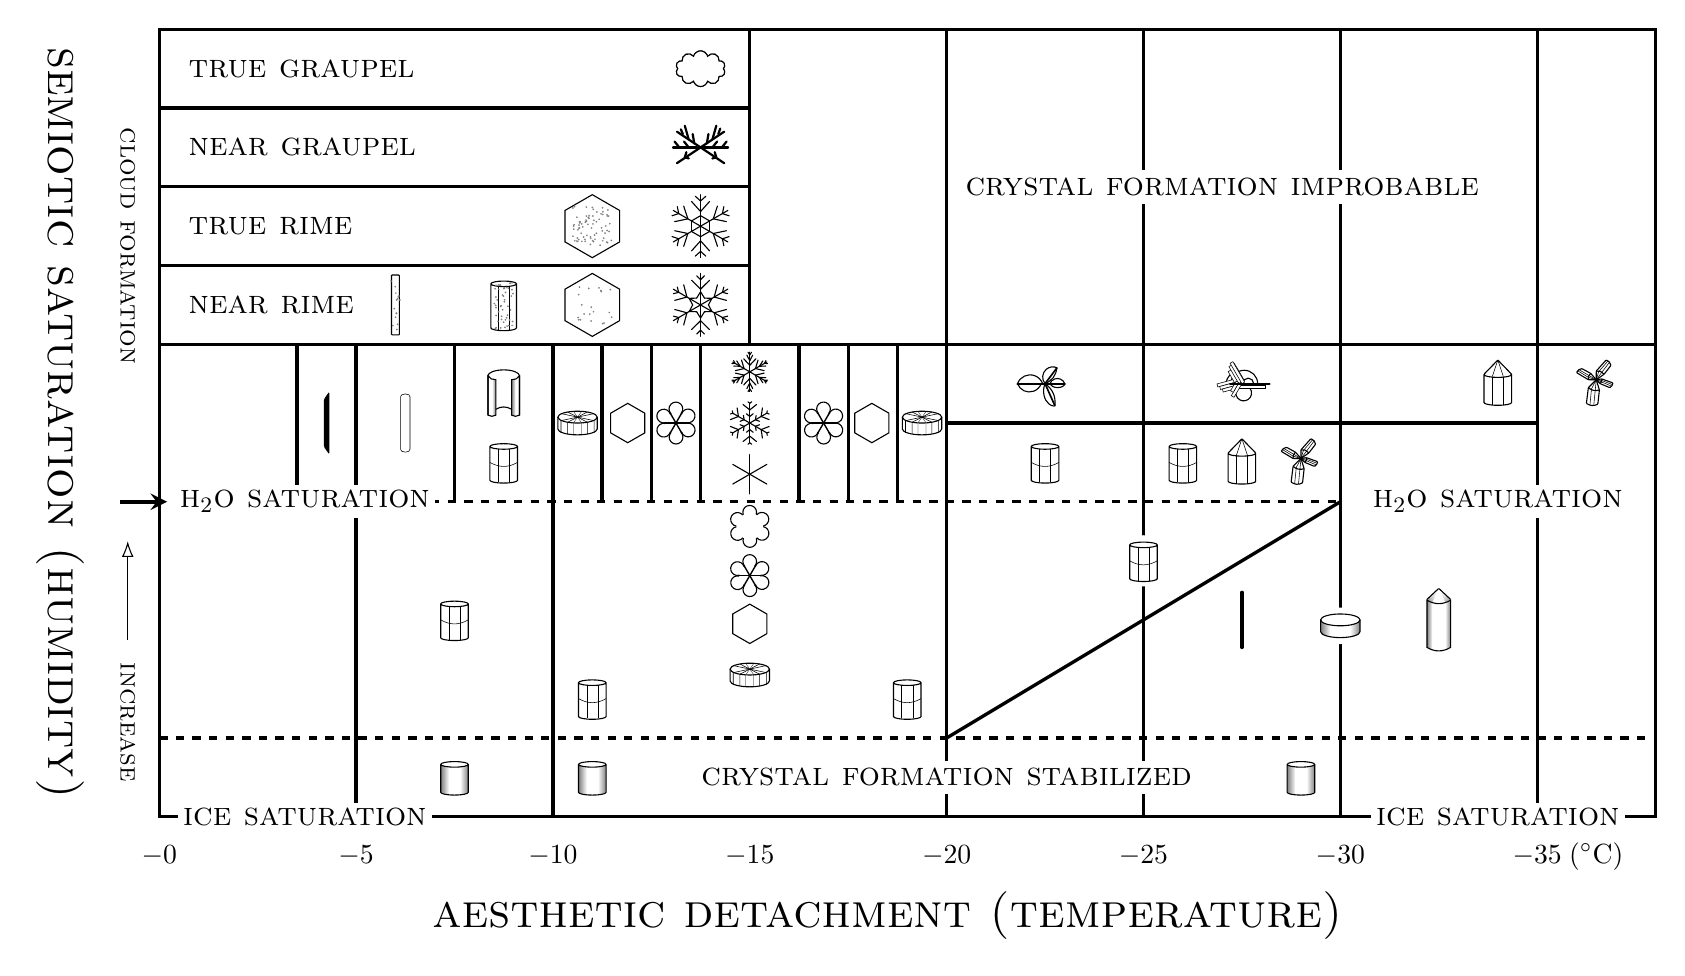
\begin{tikzpicture}
	%BOX
	\draw[very thick] (-7.5,-4) rectangle (11.5,6);
	
	%HORIZONTAL LINES
	\draw[very thick] (-7.5,5)--(0,5);		%graupel, etc.
	\draw[very thick] (-7.5,4)--(0,4);
	\draw[very thick] (-7.5,3)--(0,3);
	\draw[very thick] (-7.5,2)--(0,2);
	%
	\draw[very thick] (2.5,1)--(10,1);
	\draw[very thick,dashed] (-7,0)--(7.5,0);		%mid dashed
	\draw[very thick] (-7.5,2)--(11.5,2);			%long solid
	\draw[very thick,dashed] (-7.5,-3)--(11.5,-3);	%long dashed
	
	%VERTICAL LINES
	\draw[very thick] (0,2)--(0,6);			%rightward lines
	\draw[very thick] (2.5,-4)--(2.5,6);
	\draw[very thick] (5,-4)--(5,6);
	\draw[very thick] (7.5,-4)--(7.5,6);
	\draw[very thick] (10,-4)--(10,6);
	%
	\draw[very thick] (-2.5,-4)--(-2.5,2);	%leftward lines
	\draw[very thick] (-3.75,0)--(-3.75,2);
	\draw[very thick] (-5,-4)--(-5,2);
	\draw[very thick] (-5.75,0)--(-5.75,2);
	%
	\draw[very thick] (-1.875,0)--(-1.875,2);	%lines above circular part
	\draw[very thick] (-1.25,0)--(-1.25,2);
	\draw[very thick] (-0.625,0)--(-0.625,2);
	\draw[very thick] (0.625,0)--(0.625,2);
	\draw[very thick] (1.25,0)--(1.25,2);
	\draw[very thick] (1.875,0)--(1.875,2);
	%
	\draw[very thick] (2.5,-3)--(7.5,0);		%diagonal line
	
	%CIRCULAR PART
	\centerarc[very thick](0,0)(180:360:0.625)
	\centerarc[very thick](0,0)(180:360:1.25)
	\centerarc[very thick](0,0)(180:360:1.875)
	\centerarc[very thick](0,0)(180:360:2.5)
	
	%LABELS
	\foreach \c [count=\x from 0] in {0,5,10,15,20,25,30,35} 	%temperatures at bottom
	\node at (-7.5+2.5*\x,-4.5) {$-$\c};
	\node at (10.75,-4.5) {($^\circ$C)};	%can also use \textcelsius from textcomp package
	\node at (1.75,-5.25) {\LARGE\textsc{aesthetic detachment (temperature)}};
	%
	\node at (-8.75,1)	 {\rotatebox{-90}{\LARGE \textsc{semiotic saturation (humidity)}}};
	\node at (-7.9,3.25) {\rotatebox{-90}{\textsc{cloud formation}}};
	\node at (-7.9,-2.8) {\rotatebox{-90}{\textsc{increase}}};
		\draw[->,-{Latex[length=2mm,open]}] (-7.9,-1.75)--(-7.9,-0.5);	%OR: >=open triangle 45
		\draw[ultra thick,->,>=stealth] (-8,0)--(-7.4,0);
	%
	\node[align=left,right] at (-7.25,5.5) {\large\textsc{true graupel}};
	\node[align=left,right] at (-7.25,4.5) {\large\textsc{near graupel}};
	\node[align=left,right] at (-7.25,3.5) {\large\textsc{true rime}};
	\node[align=left,right] at (-7.25,2.5) {\large\textsc{near rime}};
	%
	\node[fill=white,inner sep=3pt] at (6,4) 	  {\large\textsc{crystal formation improbable}};
	\node[fill=white,inner sep=2pt] at (-5.65,0)  {\large\textsc{h$_2$o saturation}}; %left
	\node[fill=white,inner sep=2pt] at (-5.65,-4) {\large\textsc{ice saturation}}; %left
	\node[fill=white,inner sep=3pt] at (2.5,-3.5) {\large\textsc{crystal formation stabilized}};
	\node[fill=white,inner sep=2pt] at (9.5,0)    {\large\textsc{h$_2$o saturation}}; %right
	\node[fill=white,inner sep=2pt] at (9.5,-4)   {\large\textsc{ice saturation}}; %right
	
	%HEXAGONS
	\node[regular polygon,regular polygon sides=6,minimum size=0.5cm,draw,rotate=30] at (-1.55,1) {};
	\node[regular polygon,regular polygon sides=6,minimum size=0.5cm,draw,rotate=30] at ( 1.55,1) {};
	\node[regular polygon,regular polygon sides=6,minimum size=0.5cm,draw,rotate=30] at (0,-1.55) {};
	\node[regular polygon,regular polygon sides=6,minimum size=0.8cm,draw,rotate=30] at (-2,2.5) {};
		\foreach \p in {1,...,20} \fill[gray] (-2+0.25*rand,2.5+0.25*rand) circle (0.35pt); %frost
	\node[regular polygon,regular polygon sides=6,minimum size=0.8cm,draw,rotate=30] at (-2,3.5) {};
		\foreach \p in {1,...,75} \fill[gray] (-2+0.25*rand,3.5+0.25*rand) circle (0.35pt); %rime
	
	%SNOWFLAKES
	%rimed dendrite -- true rime (-0.625,3.5)
	\foreach \x in {0,...,5}{
	\draw[line cap=round] (-0.625,3.5)--++({0.4*cos(90+60*\x)},{0.4*sin(90+60*\x)});
	\draw[line cap=round] %hexagon in center
	({-0.625+4/30*cos(90+60*\x)},{3.5+4/30*sin(90+60*\x)})--({-0.625+4/30*cos(150+60*\x)},{3.5+4/30*sin(150+60*\x)});
	\draw[line cap=round] %middle, longest, left
	({-0.625+0.186*cos(90+60*\x)},{3.5+0.186*sin(90+60*\x)})--({-0.625+1/3*cos(110+60*\x)},{3.5+1/3*sin(110+60*\x)});
	\draw[line cap=round] %middle, longest, right
	({-0.625+0.186*cos(90+60*\x)},{3.5+0.186*sin(90+60*\x)})--({-0.625+1/3*cos(70+60*\x)},{3.5+1/3*sin(70+60*\x)});
	\draw[line cap=round] %furthest branch, left
	({-0.625+0.32*cos(90+60*\x)},{3.5+0.32*sin(90+60*\x)})--({-0.625+0.386*cos(100+60*\x)},{3.5+0.386*sin(100+60*\x)});
	\draw[line cap=round] %furthest branch, right
	({-0.625+0.32*cos(90+60*\x)},{3.5+0.32*sin(90+60*\x)})--({-0.625+0.386*cos(80+60*\x)},{3.5+0.386*sin(80+60*\x)});
		} %end of loop
	
	%frosted dendrite -- near rime (-0.625,2.5)
	\foreach \x in {0,...,5}{
	\draw[line cap=round] (-0.625,2.5)--++({0.4*cos(90+60*\x)},{0.4*sin(90+60*\x)});
	\draw[line cap=round] %closest to center, left (90+20)
	({-0.625+1/6*cos(90+60*\x)},{2.5+1/6*sin(90+60*\x)})--({-0.625+0.1*cos(120+60*\x)},{2.5+0.1*sin(120+60*\x)});
	\draw[line cap=round] %closest to center, right (90-20)
	({-0.625+1/6*cos(90+60*\x)},{2.5+1/6*sin(90+60*\x)})--({-0.625+0.1*cos(60+60*\x)},{2.5+0.1*sin(60+60*\x)});
	\draw[line cap=round] %middle, longest, left
	({-0.625+0.2*cos(90+60*\x)},{2.5+0.2*sin(90+60*\x)})--({-0.625+1/3*cos(110+60*\x)},{2.5+1/3*sin(110+60*\x)});
	\draw[line cap=round] %middle, longest, right
	({-0.625+0.2*cos(90+60*\x)},{2.5+0.2*sin(90+60*\x)})--({-0.625+1/3*cos(70+60*\x)},{2.5+1/3*sin(70+60*\x)});
	\draw[line cap=round] %furthest branch, left
	({-0.625+0.32*cos(90+60*\x)},{2.5+0.32*sin(90+60*\x)})--({-0.625+0.373*cos(97.5+60*\x)},{2.5+0.373*sin(97.5+60*\x)});
	\draw[line cap=round] %furthest branch, right
	({-0.625+0.32*cos(90+60*\x)},{2.5+0.32*sin(90+60*\x)})--({-0.625+0.373*cos(82.5+60*\x)},{2.5+0.373*sin(82.5+60*\x)});
		} %end of loop
	
	%pterideous crystal (0,1.65)
	\foreach \x in {0,...,5}{
	\draw[line cap=round] (0,1.65)--++({0.25*cos(90+60*\x)},{0.25*sin(90+60*\x)});
	\draw[line cap=round] %closest to center, left (90+20)
	({25/300*cos(90+60*\x)},{1.65+25/300*sin(90+60*\x)})--({0.183*cos(115+60*\x)},{1.65+0.183*sin(115+60*\x)});
	\draw[line cap=round] %closest to center, right (90-20)
	({25/300*cos(90+60*\x)},{1.65+25/300*sin(90+60*\x)})--({0.183*cos(65+60*\x)},{1.65+0.183*sin(65+60*\x)});
	\draw[line cap=round] %middle, longest, left
	({0.1416*cos(90+60*\x)},{1.65+0.1416*sin(90+60*\x)})--({0.216*cos(100+60*\x)},{1.65+0.216*sin(100+60*\x)});
	\draw[line cap=round] %middle, longest, right
	({0.1416*cos(90+60*\x)},{1.65+0.1416*sin(90+60*\x)})--({0.216*cos(80+60*\x)},{1.65+0.216*sin(80+60*\x)});
	\draw[line cap=round] %tip of snowflake left
	({0.216*cos(90+60*\x)},{1.65+0.216*sin(90+60*\x)})--({0.25*cos(95+60*\x)},{1.65+0.25*sin(95+60*\x)});
	\draw[line cap=round] %tip of snowflake, right
	({0.216*cos(90+60*\x)},{1.65+0.216*sin(90+60*\x)})--({0.25*cos(85+60*\x)},{1.65+0.25*sin(85+60*\x)});
		} %end of loop
	
	%dendritic crystal (0,1)
	\foreach \x in {0,...,5}{
	\draw[line cap=round] (0,1)--++({0.25*cos(90+60*\x)},{0.25*sin(90+60*\x)});
	\draw[line cap=round] %closest to center, left (90+20)
	({25/300*cos(90+60*\x)},{1+25/300*sin(90+60*\x)})--({0.125*cos(110+60*\x)},{1+0.125*sin(110+60*\x)});
	\draw[line cap=round] %closest to center, right (90-20)
	({25/300*cos(90+60*\x)},{1+25/300*sin(90+60*\x)})--({0.125*cos(70+60*\x)},{1+0.125*sin(70+60*\x)});
	\draw[line cap=round] %middle, longest, left
	({50/300*cos(90+60*\x)},{1+50/300*sin(90+60*\x)})--({0.25*cos(110+60*\x)},{1+0.25*sin(110+60*\x)});
	\draw[line cap=round] %middle, longest, right
	({50/300*cos(90+60*\x)},{1+50/300*sin(90+60*\x)})--({0.25*cos(70+60*\x)},{1+0.25*sin(70+60*\x)});
	\draw[line cap=round] %tip of snowflake left
	({0.25*cos(90+60*\x)},{1+0.25*sin(90+60*\x)})--({0.271*cos(95+60*\x)},{1+0.271*sin(95+60*\x)});
	\draw[line cap=round] %tip of snowflake, right
	({0.25*cos(90+60*\x)},{1+0.25*sin(90+60*\x)})--({0.271*cos(85+60*\x)},{1+0.271*sin(85+60*\x)});
		} %end of loop
	
	%stellar crystal (0,0.35)
	\foreach \x in {0,...,5} \draw[line cap=round] (0,.35)--++({.25*cos(90+60*\x)},{.25*sin(90+60*\x)});
	
	%FROSTED NEEDLE -- at (-4.5,2.5)
	\draw[rounded corners=0.25pt] (-4.5-0.05,2.5-0.38) rectangle (-4.5+0.05,2.5+0.38);
	\foreach \p in {1,...,15} \fill[gray] (-4.5+0.075*rand,2.5+0.32*rand) circle (0.35pt); %dots
	
	%FROSTED COLUMN -- at (-3.125,2.5)
	\node[cylinder,draw,shape border rotate=90,shape aspect=.3,minimum height=0.63cm,minimum width=0.325cm] at (-3.125+0,2.5-0.05) {};
	\draw[very thin] (-3.125-0.07,2.5-0.32)--(-3.125-0.07,2.5+0.23);
	\draw[very thin] (-3.125+0.07,2.5-0.32)--(-3.125+0.07,2.5+0.23);
	\foreach \p in {1,...,50} \fill[gray] (-3.125+0.12*rand,2.5+0.3*rand) circle (0.35pt); %dots
	
	%AGGREGATE GRAUPEL -- at (-0.625,4.5)
	\draw[thick,line cap=round] (-0.625-0.35,4.5)--(-0.625+0.35,4.5);
		\draw[thick,line cap=round] (-0.625-0.27,4.5)--(-0.625-0.33,4.5+0.075);
		\draw[thick,line cap=round] (-0.625-0.15,4.5)--(-0.625-0.21,4.5+0.075);
		\draw[thick,line cap=round] (-0.625+0.15,4.5)--(-0.625+0.21,4.5+0.075);
		\draw[thick,line cap=round] (-0.625+0.27,4.5)--(-0.625+0.33,4.5+0.075);
	\draw[thick,line cap=round] (-0.625-0.3,4.5-0.2)--(-0.625+0.3,4.5+0.2);	%SW--NE
		\draw[thick,line cap=round] (-0.625-0.2,4.5-0.125)--(-0.625-0.18,4.5-0.06);	%SW nub, top
		\draw[thick,line cap=round] (-0.625-0.2,4.5-0.125)--(-0.625-0.15,4.5-0.14);	%SW nub, bottom
		\draw[thick,line cap=round] (-0.625-0.08,4.5+0.05)--(-0.625-0.1,4.5+0.17);	%near origin
		\draw[thick,line cap=round] (-0.625-0.15,4.5+0.1)--(-0.625-0.2,4.5+0.275);	%long branch
		\draw[thick,line cap=round] (-0.625-0.225,4.5+0.17)--(-0.625-0.25,4.5+0.23);%nub at tip
	\draw[thick,line cap=round] (-0.625+0.3,4.5-0.2)--(-0.625-0.3,4.5+0.2);	%SE--NW
		\draw[thick,line cap=round] (-0.625+0.2,4.5-0.125)--(-0.625+0.18,4.5-0.06);	%SE nub, top
		\draw[thick,line cap=round] (-0.625+0.2,4.5-0.125)--(-0.625+0.15,4.5-0.14);	%SE nub, bottom
		\draw[thick,line cap=round] (-0.625+0.08,4.5+0.05)--(-0.625+0.1,4.5+0.17);	%near origin
		\draw[thick,line cap=round] (-0.625+0.15,4.5+0.1)--(-0.625+0.2,4.5+0.275);	%long branch
		\draw[thick,line cap=round] (-0.625+0.225,4.5+0.17)--(-0.625+0.25,4.51+0.23);	%nub at tip
	
	%HOLLOW COLUMNS
	\node[cylinder,draw,shape border rotate=90,shape aspect=.3,minimum height=0.5cm,minimum width=0.35cm] at (-3.125+0,0.5-0.05) {};	%at (-3.125,0.5)
	\draw[very thin] (-3.125-0.175,0.5-0) to[bend right] (-3.125+0.175,0.5-0);
	\draw[very thin] (-3.125-0.07,0.5-0.25)--(-3.125-0.07,0.5+0.17);	%vertical line, left
	\draw[very thin] (-3.125+0.07,0.5-0.25)--(-3.125+0.07,0.5+0.17);	%vertical line, right
	%
	\node[cylinder,draw,shape border rotate=90,shape aspect=.3,minimum height=0.5cm,minimum width=0.35cm] at (-3.75+0,-1.5-0.05) {};	%at (-3.75,-1.5)
	\draw[very thin] (-3.75-0.175,-1.5-0) to[bend right] (-3.75+0.175,-1.5-0);
	\draw[very thin] (-3.75-0.07,-1.5-0.25)--(-3.75-0.07,-1.5+0.17);	%vertical line, left
	\draw[very thin] (-3.75+0.07,-1.5-0.25)--(-3.75+0.07,-1.5+0.17);	%vertical line, right
	%
	\node[cylinder,draw,shape border rotate=90,shape aspect=.3,minimum height=0.5cm,minimum width=0.35cm] at (-2+0,-2.5-0.05) {};	%at (-2,-2.5)
	\draw[very thin] (-2-0.175,-2.5-0) to[bend right] (-2+0.175,-2.5-0);
	\draw[very thin] (-2-0.07,-2.5-0.25)--(-2-0.07,-2.5+0.17);	%vertical line, left
	\draw[very thin] (-2+0.07,-2.5-0.25)--(-2+0.07,-2.5+0.17);	%vertical line, right
	%
	\node[cylinder,draw,shape border rotate=90,shape aspect=.3,minimum height=0.5cm,minimum width=0.35cm] at (2+0,-2.5-0.05) {};	%at (2,-2.5)
	\draw[very thin] (2-0.175,-2.5-0) to[bend right] (2+0.175,-2.5-0);
	\draw[very thin] (2-0.07,-2.5-0.25)--(2-0.07,-2.5+0.17);	%vertical line, left
	\draw[very thin] (2+0.07,-2.5-0.25)--(2+0.07,-2.5+0.17);	%vertical line, right
	%
	\node[cylinder,draw,shape border rotate=90,shape aspect=.3,minimum height=0.5cm,minimum width=0.35cm] at (3.75+0,0.5-0.05) {};	%at (3.75,0.5)
	\draw[very thin] (3.75-0.175,0.5-0) to[bend right] (3.75+0.175,0.5-0);
	\draw[very thin] (3.75-0.07,0.5-0.25)--(3.75-0.07,0.5+0.17);	%vertical line, left
	\draw[very thin] (3.75+0.07,0.5-0.25)--(3.75+0.07,0.5+0.17);	%vertical line, right
	%
	\node[cylinder,draw,shape border rotate=90,shape aspect=.3,minimum height=0.5cm,minimum width=0.35cm] at (5.5+0,0.5-0.05) {};	%at (5.5,0.5)
	\draw[very thin] (5.5-0.175,0.5-0) to[bend right] (5.5+0.175,0.5-0);
	\draw[very thin] (5.5-0.07,0.5-0.25)--(5.5-0.07,0.5+0.17);	%vertical line, left
	\draw[very thin] (5.5+0.07,0.5-0.25)--(5.5+0.07,0.5+0.17);	%vertical line, right
	%
	\fill[white] (5,-0.75) circle (0.325);
	\node[cylinder,draw,shape border rotate=90,shape aspect=.3,minimum height=0.5cm,minimum width=0.35cm] at (5+0,-0.75-0.05) {};	%at (5,-0.75)
	\draw[very thin] (5-0.175,-0.75-0) to[bend right] (5+0.175,-0.75-0);
	\draw[very thin] (5-0.07,-0.75-0.25)--(5-0.07,-0.75+0.17);	%vertical line, left
	\draw[very thin] (5+0.07,-0.75-0.25)--(5+0.07,-0.75+0.17);	%vertical line, right
	
	%SECTORED PLATE
	\foreach \x in {0,...,5}{	%at (-0.9375,1)
	\draw ({-0.9375+2/3*0.2*cos(90+28+60*\x)},{1+2/3*0.2*sin(90+28+60*\x)}) arc (180+45+60*\x:0-42+60*\x:0.087cm);
	\draw[line width=0.5] ({-0.9375+2/3*0.22*cos(90+30+60*\x)},{1+2/3*0.22*sin(90+30+60*\x)}) -- (-0.9375,1);
		}	%end of loop
	%
	\foreach \x in {0,...,5}{	%at (0.9375,1)
	\draw ({0.9375+2/3*0.2*cos(90+28+60*\x)},{1+2/3*0.2*sin(90+28+60*\x)}) arc (180+45+60*\x:0-42+60*\x:0.087cm);
	\draw[line width=0.5] ({0.9375+2/3*0.22*cos(90+30+60*\x)},{1+2/3*0.22*sin(90+30+60*\x)}) -- (0.9375,1);
		}	%end of loop
	%
	\foreach \x in {0,...,5}{	%at (0,-0.9375)
		\draw ({0+2/3*0.2*cos(90+28+60*\x)},{-0.9375+2/3*0.2*sin(90+28+60*\x)}) arc (180+45+60*\x:0-42+60*\x:0.087cm);
		\draw[line width=0.5] ({0+2/3*0.22*cos(90+30+60*\x)},{-0.9375+2/3*0.22*sin(90+30+60*\x)})--(0,-0.9375);
	}	%end of loop
	%BRANCHED PLATE
	\foreach \x in {0,...,5}{	%at (0,-0.3125)
		\draw ({0+2/3*0.2*cos(90+28+60*\x)},{-0.3125+2/3*0.2*sin(90+28+60*\x)}) arc (180+45+60*\x:0-42+60*\x:0.087cm);
		\draw[line width=0.5] ({0+2/3*0.22*cos(90+30+60*\x)},{-0.3125+2/3*0.22*sin(90+30+60*\x)})--(0,-0.3125);
	}	%end of loop
	\fill[white] (0,-0.3125) circle (0.17);
	
	%HOLLOW PLATE
	\draw (-2.1875,1.075) ellipse (0.25 and 0.075);	%at (-2.1875,1.075)
	\draw (-2.1875+0.25,1.075-0)--(-2.1875+0.25,1.075-0.15) arc (0:-180:0.25 and 0.075)--(-2.1875-0.25,1.075-0);
	\draw[very thin] (-2.1875+0,1.075-0)--(-2.1875-0.125,1.075+0.065);
	\draw[very thin] (-2.1875+0,1.075-0)--(-2.1875+0.125,1.075+0.065);
	\draw[very thin] (-2.1875-0.125,1.075-0.215)--(-2.1875-0.125,1.075-0.065)--(-2.1875,1.075-0);
	\draw[very thin] (-2.1875+0.125,1.075-0.215)--(-2.1875+0.125,1.075-0.065)--(-2.1875,1.075-0);
	%
	\draw[ultra thin] (-2.1875,1.075-0)--(-2.1875-0.05,1.075+0.07);	%innermost vertical lines
	\draw[ultra thin] (-2.1875,1.075-0)--(-2.1875+0.05,1.075+0.07);
	\draw[ultra thin] (-2.1875-0.05,1.075-0.22)--(-2.1875-0.05,1.075-0.07)--(-2.1875,1.075-0);
	\draw[ultra thin] (-2.1875+0.05,1.075-0.22)--(-2.1875+0.05,1.075-0.07)--(-2.1875,1.075-0);
	%
	\draw[very thin] (-2.1875,1.075-0)--(-2.1875-0.21,1.075+0.045);
	\draw[very thin] (-2.1875,1.075-0)--(-2.1875+0.21,1.075+0.045);
	\draw[very thin] (-2.1875-0.21,1.075-0.2)--(-2.1875-0.21,1.075-0.045)--(-2.1875,1.075-0);
	\draw[very thin] (-2.1875+0.21,1.075-0.2)--(-2.1875+0.21,1.075-0.045)--(-2.1875,1.075-0);
	%
	%
	\draw (2.1875,1.075) ellipse (0.25 and 0.075);	%at (2.1875,1.075)
	\draw (2.1875+0.25,1.075-0)--(2.1875+0.25,1.075-0.15) arc (0:-180:0.25 and 0.075)--(2.1875-0.25,1.075-0);
	\draw[very thin] (2.1875+0,1.075-0)--(2.1875-0.125,1.075+0.065);
	\draw[very thin] (2.1875+0,1.075-0)--(2.1875+0.125,1.075+0.065);
	\draw[very thin] (2.1875-0.125,1.075-0.215)--(2.1875-0.125,1.075-0.065)--(2.1875,1.075-0);
	\draw[very thin] (2.1875+0.125,1.075-0.215)--(2.1875+0.125,1.075-0.065)--(2.1875,1.075-0);
	%
	\draw[ultra thin] (2.1875,1.075-0)--(2.1875-0.05,1.075+0.07);	%innermost vertical lines
	\draw[ultra thin] (2.1875,1.075-0)--(2.1875+0.05,1.075+0.07);
	\draw[ultra thin] (2.1875-0.05,1.075-0.22)--(2.1875-0.05,1.075-0.07)--(2.1875,1.075-0);
	\draw[ultra thin] (2.1875+0.05,1.075-0.22)--(2.1875+0.05,1.075-0.07)--(2.1875,1.075-0);
	%
	\draw[very thin] (2.1875,1.075-0)--(2.1875-0.21,1.075+0.045);
	\draw[very thin] (2.1875,1.075-0)--(2.1875+0.21,1.075+0.045);
	\draw[very thin] (2.1875-0.21,1.075-0.2)--(2.1875-0.21,1.075-0.045)--(2.1875,1.075-0);
	\draw[very thin] (2.1875+0.21,1.075-0.2)--(2.1875+0.21,1.075-0.045)--(2.1875,1.075-0);
	%
	%
	\draw (0,-2.125) ellipse (0.25 and 0.075);
	\draw (0.25,-2.125-0)--(0.25,-2.125-0.15) arc (0:-180:0.25 and 0.075)--(-0.25,-2.125-0);
	\draw[very thin] (0,-2.125-0)--(-0.125,-2.125+0.065);
	\draw[very thin] (0,-2.125-0)--( 0.125,-2.125+0.065);
	\draw[very thin] (-0.125,-2.125-0.215)--(-0.125,-2.125-0.065)--(0,-2.125-0);
	\draw[very thin] ( 0.125,-2.125-0.215)--( 0.125,-2.125-0.065)--(0,-2.125-0);
	%
	\draw[ultra thin] (0,-2.125-0)--(-0.05,-2.125+0.07);	%innermost vertical lines
	\draw[ultra thin] (0,-2.125-0)--( 0.05,-2.125+0.07);
	\draw[ultra thin] (-0.05,-2.125-0.22)--(-0.05,-2.125-0.07)--(0,-2.125-0);
	\draw[ultra thin] ( 0.05,-2.125-0.22)--( 0.05,-2.125-0.07)--(0,-2.125-0);
	%
	\draw[very thin] (0,-2.125-0)--(-0.21,-2.125+0.045);
	\draw[very thin] (0,-2.125-0)--( 0.21,-2.125+0.045);
	\draw[very thin] (-0.21,-2.125-0.2)--(-0.21,-2.125-0.045)--(0,-2.125-0);
	\draw[very thin] ( 0.21,-2.125-0.2)--( 0.21,-2.125-0.045)--(0,-2.125-0);
	
	%SOLID COLUMN
	\shade[left color=gray,right color=white]	%at (-3.75,-3.5)
	(-3.75-0.07,-3.5-0.23)--(-3.75-0.175,-3.5-0.19)--(-3.75-0.175,-3.5+0.16)--(-3.75-0.07,-3.5+0.13)--cycle; %L
	\shade[left color=white,right color=gray] (-3.75+0.07,-3.5-0.23)--(-3.75+0.175,-3.5-0.19)--(-3.75+0.175,-3.5+0.16)--(-3.75+0.07,-3.5+0.13)--cycle; %R
	\node[cylinder,draw,shape border rotate=90,shape aspect=.3,minimum height=0.425cm,minimum width=0.35cm] at (-3.75+0,-3.5-0.05) {};
	%
	\shade[left color=gray,right color=white]	%at (-2,-3.5)
	(-2-0.07,-3.5-0.23)--(-2-0.175,-3.5-0.19)--(-2-0.175,-3.5+0.16)--(-2-0.07,-3.5+0.13)--cycle; %L
	\shade[left color=white,right color=gray] (-2+0.07,-3.5-0.23)--(-2+0.175,-3.5-0.19)--(-2+0.175,-3.5+0.16)--(-2+0.07,-3.5+0.13)--cycle; %R
	\node[cylinder,draw,shape border rotate=90,shape aspect=.3,minimum height=0.425cm,minimum width=0.35cm] at (-2+0,-3.5-0.05) {};
	%
	\shade[left color=gray,right color=white]	%at (7,-3.5)
	(7-0.07,-3.5-0.23)--(7-0.175,-3.5-0.19)--(7-0.175,-3.5+0.16)--(7-0.07,-3.5+0.13)--cycle; %L
	\shade[left color=white,right color=gray] (7+0.07,-3.5-0.23)--(7+0.175,-3.5-0.19)--(7+0.175,-3.5+0.16)--(7+0.07,-3.5+0.13)--cycle; %R
	\node[cylinder,draw,shape border rotate=90,shape aspect=.3,minimum height=0.425cm,minimum width=0.35cm] at (7+0,-3.5-0.05) {};
	
	%SCROLL -- at (-3.125,1.5)
	\shade[left color=white,right color=gray] %shade left
	(-3.125-.1,1.35+0.2)--(-3.125-.15,1.35+0.22)--(-3.125-.15,1.35-0.27)--(-3.125-.1,1.35-0.25)--cycle;
	\shade[left color=gray,right color=white] %shade right
	(-3.125+0.1,1.35+0.2)--(-3.125+0.15,1.35+0.22)--(-3.125+0.15,1.35-0.27)--(-3.125+0.1,1.35-0.25)--cycle;
	\draw (-3.125-0.2,1.35-0.25)--(-3.125-0.2,1.35+0.25) arc (180:0:0.2 and 0.075)--(-3.125+0.2,1.35-0.25);
	\draw (-3.125-.2,1.35+0.25) to[bend right] (-3.125-.1,1.35+0.2)--(-3.125-.1,1.35-0.25) to[bend left] (-3.125-.2,1.35-0.25)--cycle;
	\draw (-3.125+0.2,1.35+0.25) to[bend left] (-3.125+0.1,1.35+0.2)--(-3.125+0.1,1.35-0.25) to[bend right] (-3.125+0.2,1.35-0.25)--cycle;	
	\draw (-3.125-0.1,1.35-0.175) to[bend left] (-3.125+0.1,1.35-0.175); %bottom bend in center
	
	%ELEMENTARY SHEATH -- at (-4.5,1)
	\filldraw[fill=white,draw=black,very thin,rounded corners=0.5pt] (-4.375-0.12/2,1-0.35)--++(0,2*0.35) to[bend left] ++(0.12,0) -- ++(0,-2*0.35) to[bend left] ++(-0.12,0) -- cycle;
	
	%ELEMENTARY NEEDLE -- at (-5.375,1)
	\fill[rounded corners=0.5pt] (-5.375-0.07/2,1-0.25)--++(0,0.55)--++(0.07,0.1)--++(0,-0.8)--++(-0.07,0.1)--cycle;
	
	%COLUMNAR NEEDLE -- at (6.25,-1.5)
	\draw[very thick,line cap=round] (6.25,-1.5-0.35)--++(0,0.7);
	
	%CLOUD
	\node[cloud, draw, fill=gray!1, aspect=1.75] at (-0.625,5.5) {};
	\node[cloud, draw, fill=gray!1, aspect=1.75] at (-0.625,5.5) {};
	
	%HOLLOW BULLET
	\node[cylinder,draw,shape border rotate=90,shape aspect=.3,minimum height=0.425cm,minimum width=0.35cm] at (6.25,0.45-0.05) {}; %(6.25,0.45)
	\draw[white,line width=1.1pt] (6.25-0.145,0.45+0.193)--(6.25+0.145,0.45+0.193); %coverup
	\draw[white,semithick] (6.25-0.165,0.45+0.18)--(6.25+0.165,0.45+0.18);
	\draw[rounded corners=.25pt] (6.25-0.17,0.45+0.175)--(6.25,0.45+0.35)--(6.25+0.17,0.45+0.175);
	\draw[very thin,rounded corners=0.25pt] (6.25-0.07,0.45+0.14)--(6.25,0.45+0.35)--(6.25+0.07,0.45+0.14);	%point, low
	\draw[very thin] (6.25-0.07,0.45-0.22)--(6.25-0.07,0.45+0.14);	%left vertical line
	\draw[very thin] (6.25+0.07,0.45-0.22)--(6.25+0.07,0.45+0.14);	%right vertical line
	%
	\node[cylinder,draw,shape border rotate=90,shape aspect=.3,minimum height=0.425cm,minimum width=0.35cm] at (9.5,1.45-0.05) {}; %(9.75,1.45)
	\draw[white,line width=1.1pt] (9.5-0.145,1.45+0.193)--(9.5+0.145,1.45+0.193);
	\draw[white,semithick] (9.5-0.165,1.45+0.18)--(9.5+0.165,1.45+0.18);
	\draw[rounded corners=.25pt] (9.5-.17,1.45+0.175)--(9.5,1.45+0.35)--(9.5+0.17,1.45+.175); %top
	\draw[very thin,rounded corners=0.25pt] (9.5-0.07,1.45+0.14)--(9.5,1.45+0.35)--(9.5+0.07,1.45+0.14);	%point, low
	\draw[very thin] (9.5-0.07,1.45-0.22)--(9.5-0.07,1.45+0.14);	%left vertical line
	\draw[very thin] (9.5+0.07,1.45-0.22)--(9.5+0.07,1.45+0.14);	%right vertical line
	
	%SOLID PLATE -- at (7.5,-1.5)
	\filldraw[white] (7.5,-1.575) circle (0.225cm);
	\shade[left color=gray,right color=white] (7.5-0.25,-1.5-0)--(7.5-0.25,-1.5-0.15) arc (180:240:0.25 and 0.075) -- ++(0,0.15) arc (-120:-175:0.25 and 0.075) -- cycle;	%shading left
	\shade[left color=white,right color=gray] (7.5+0.125,-1.5-0.065)--(7.5+0.125,-1.5-0.215) arc (300:360:0.25 and 0.075) -- ++(0,0.145) arc (-5:-60:0.25 and 0.075) -- cycle;	%shading right
	\draw (7.5,-1.5) ellipse (0.25 and 0.075);
	\draw (7.5-0.25,-1.5-0)--(7.5-0.25,-1.5-0.15) arc (180:360:0.25 and 0.075) --(7.5+0.25,-1.5-0);
	
	%SOLID BULLET -- at (8.75,-1.5)
	%shading, left rectangle
	\shade[left color=gray,right color=white] (8.75-0.08,-1.5-0.39)--(8.75-0.15,-1.5-0.35)--(8.75-0.15,-1.5+0.26)--(8.75-0.08,-1.5+0.225)--(8.75-0.15,-1.5+0.26)--(8.75-0.08,-1.5+0.225)--cycle;
	%shading, left triangle
	\shade[lower left=gray,upper right=white] (8.75-0.15,-1.5+0.26)--(8.75+0,-1.5+0.4)--(8.75-0.08,-1.5+0.225)--cycle;
	%shading, right rectangle
	\shade[left color=white,right color=gray] (8.75+.08,-1.5-0.39)--(8.75+.15,-1.5-0.35)--(8.75+.15,-1.5+0.26)--(8.75+.08,-1.5+0.225)--(8.75+.15,-1.5+0.26)--(8.75+.08,-1.5+.225)--cycle;
	%shading, right triangle
	\shade[lower right=gray,upper left=white] (8.75+0.15,-1.5+0.26)--(8.75+0,-1.5+0.4)--(8.75+0.08,-1.5+0.225)--cycle;
	%
	\draw[rounded corners=0.25pt] (8.75-0.15,-1.5+0.26)--(8.75+0,-1.5+0.4)--(8.75+0.15,-1.5+0.26);		%point, top
	\draw (8.75-0.15,-1.5-0.35)--(8.75-0.15,-1.5+0.25) to[bend right] (8.75+0.15,-1.5+0.25) -- 
	(8.75+0.15,-1.5-0.35) to[bend left] (8.75-0.15,-1.5-0.35)--cycle;
	
	%PLANAR AGGREGATE -- at (3.75,1.5)
	\draw[thick,line cap=round] (3.75-0.35,1.5)--(3.75+0.25,1.5);
		\draw[semithick,line cap=round] (3.75+0,1.5)--(3.75+0.15,1.5+0.2);	%0--NE
		\draw[semithick,line cap=round] (3.75+0,1.5)--(3.75+0.125,1.5-0.28);	%0--SE
	\draw (3.75-0.35,1.5) arc (180-20:0+20:0.17cm);		%left petal,top
	\draw (3.75-0.35,1.5) arc (180+20:360-20:0.16cm);		%left petal,bottom
	\draw (3.75+0.25,1.5) arc (0+20:180-20:0.1cm);			%right petal,top
	\draw (3.75+0.25,1.5) arc (360:180:0.09cm and 0.05cm);	%right petal,bottom
	\draw (3.75+0,1.5) arc (220:65:0.13cm);					%NE petal, left
	\draw (3.75+0,1.5) to[bend right] (3.75+0.15,1.5+0.2);	%NE petal, right
	\draw (3.75+0,1.5) arc (150:270:0.14cm and 0.19cm);		%SE petal, left
	\draw (3.75+0,1.5) to[bend left] (3.75+0.125,1.5-0.28);	%SE petal, right
	
	%COLUMNAR CLUSTER -- at (6.25,1.5)
	\draw (6.25+0.2,1.5) arc (0:180:0.17cm);		%top big arc
	\draw (6.25+0.15,1.5) arc (0:180:0.07cm);		%top little arc
	\draw (6.25+0.04,1.5-.02) arc (80:-180:0.1cm);	%bottom arc
	\draw (6.25-0.2,1.5) arc (180:90:0.15cm);		%leftmost arc
	%
	\filldraw[fill=white,draw=black,very thin] (6.25-.1,1.5-0.02) rectangle (6.25+0.3,1.5-.06); %--
	%
	\filldraw[fill=white,draw=black,very thin,rotate around={15:(6.25-0.08,1.5+0.06)}] (6.25-0.08,1.5+0.06) rectangle (6.25-0.325,1.5+0.02);	%leftmost bars
	\filldraw[fill=white,draw=black,very thin,rotate around={15:(6.25-0.08,1.5+0.06)}] (6.25-0.08,1.5+0.02) rectangle (6.25-0.3,1.5-0.02);
	\filldraw[fill=white,draw=black,very thin,rotate around={15:(6.25-0.08,1.5+0.06)}] (6.25-0.08,1.5-0.02) rectangle (6.25-0.275,1.5-0.06);
	%
	\filldraw[fill=white,draw=black,very thin,rotate around={30:(6.25-0.04,1.5)}] (6.25-0.08,1.5+.01) rectangle (6.25+0.04,1.5+0.2); %upper bars, shortest
	\filldraw[fill=white,draw=black,very thin,rotate around={30:(6.25-0.04,1.5)}] (6.25-0.04,1.5) rectangle (6.25+0.04,1.5+0.25);
	\filldraw[fill=white,draw=black,very thin,rotate around={30:(6.25+0,1.5)}] (6.25+0,1.5) rectangle (6.25+0.04,1.5+0.3); %longest
	%
	\filldraw[fill=white,draw=black,very thin,rotate around={150:(6.25+0,1.5)}] (6.25+0,1.5+.01) rectangle (6.25+0.04,1.5+0.2); %lower bars, longest
	\filldraw[fill=white,draw=black,very thin,rotate around={150:(6.25+0,1.5)}] (6.25+0.08,1.5+.01) rectangle (6.25+0.04,1.5+0.15);
	%
	\draw[thick,line cap=round] (6.25-0.15,1.5)--(6.25+0.35,1.5);	%horizontal line
	
	%BULLET COMBINATION
	%at (7,0.55)
	%bottom
	\draw[rounded corners=0.25pt] (7+0,0.55)--(7-0.1,0.55-0.1)--(7-0.125,0.55-0.3) to[bend right] (7+0.02,0.55-0.31) -- (7+0.04,0.55-0.13)--cycle;
	\draw (7-0.1,0.55-0.1) to[bend right] (7+0.04,0.55-0.13);
	\draw[very thin] (7+0,0.55)--(7-0.06,0.55-0.115)--(7-0.08,0.55-0.32);	%left
	\draw[very thin] (7+0,0.55)--(7-0.0313,0.55-0.323);	%right
	%
	%leftmost
	\draw[rounded corners=0.25pt] (7+0,0.55)--(7-0.1,0.55)--(7-0.25,0.55+0.09) to[bend left] (7-0.18,0.55+0.14) --(7-0.07,0.55+0.08)--cycle;
	\draw (7-0.1,0.55) to[bend left] (7-0.07,0.55+0.08);
	\draw[very thin] (7+0,0.55)--(7-0.215,0.55+0.125);	%right
	\draw[very thin] (7+0,0.55)--(7-0.1,0.55+0.03)--(7-0.23,0.55+0.11);	%left
	%
	%top
	\draw[rounded corners=0.25pt] (7+0,0.55)--(7+0,0.55+0.11)--(7+0.125,0.55+0.25) to[bend left] (7+0.185,0.55+0.18)--(7+0.1,0.55+0.07)--cycle;
	\draw (7+0,0.55+0.11) to[bend left] (7+0.1,0.55+0.07);
	\draw[very thin] (7+0,0.55)--(7+0.03,0.55+0.1)--(7+0.15,0.55+0.24);
	\draw[very thin] (7+0,0.55)--(7+0.17,0.55+0.225);
	%
	%right
	\draw[rounded corners=0.25pt] (7+0,0.55)--(7+0.07,0.55+0.01)--(7+0.21,0.55-0.04) to[bend left] (7+0.17,0.55-0.1)--(7+0.05,0.55-0.05)--cycle;
	\draw (7+0.07,0.55+0.01) to[bend left] (7+0.05,0.55-0.05);
	\draw[very thin] (7+0,0.55)--(7+0.07,0.55-0.01)--(7+0.2,0.55-0.06);
	\draw[very thin] (7+0,0.55)--(7+0.19,0.55-0.08);
	%
	%
	%at (10.75,1.55)
	%bottom
	\draw[rounded corners=0.25pt] (10.75+0,1.55)--(10.75-0.1,1.55-0.1)--(10.75-0.125,1.55-0.3) to[bend right] (10.75+0.02,1.55-0.31) -- (10.75+0.04,1.55-0.13)--cycle;
	\draw (10.75-0.1,1.55-0.1) to[bend right] (10.75+0.04,1.55-0.13);
	\draw[very thin] (10.75+0,1.55)--(10.75-0.06,1.55-0.115)--(10.75-0.08,1.55-0.32);	%left
	\draw[very thin] (10.75+0,1.55)--(10.75-0.0313,1.55-0.323);	%right
	%
	%leftmost
	\draw[rounded corners=0.25pt] (10.75+0,1.55)--(10.75-0.1,1.55)--(10.75-0.25,1.55+0.09) to[bend left] (10.75-0.18,1.55+0.14) --(10.75-0.07,1.55+0.08)--cycle;
	\draw (10.75-0.1,1.55) to[bend left] (10.75-0.07,1.55+0.08);
	\draw[very thin] (10.75+0,1.55)--(10.75-0.215,1.55+0.125);	%right
	\draw[very thin] (10.75+0,1.55)--(10.75-0.1,1.55+0.03)--(10.75-0.23,1.55+0.11);	%left
	%
	%top
	\draw[rounded corners=0.25pt] (10.75+0,1.55)--(10.75+0,1.55+0.11)--(10.75+0.125,1.55+0.25) to[bend left] (10.75+0.185,1.55+0.18)--(10.75+0.1,1.55+0.07)--cycle;
	\draw (10.75+0,1.55+0.11) to[bend left] (10.75+0.1,1.55+0.07);
	\draw[very thin] (10.75+0,1.55)--(10.75+0.03,1.55+0.1)--(10.75+0.15,1.55+0.24);
	\draw[very thin] (10.75+0,1.55)--(10.75+0.17,1.55+0.225);
	%
	%right
	\draw[rounded corners=0.25pt] (10.75+0,1.55)--(10.75+0.07,1.55+0.01)--(10.75+0.21,1.55-0.04) to[bend left] (10.75+0.17,1.55-0.1)--(10.75+0.05,1.55-0.05)--cycle;
	\draw (10.75+0.07,1.55+0.01) to[bend left] (10.75+0.05,1.55-0.05);
	\draw[very thin] (10.75+0,1.55)--(10.75+0.07,1.55-0.01)--(10.75+0.2,1.55-0.06);
	\draw[very thin] (10.75+0,1.55)--(10.75+0.19,1.55-0.08);
	
	\end{tikzpicture}
	
\end{document}